% Figure: layout of the family measure mu_k (drawn for k = 11; one unit = 0.42 cm)
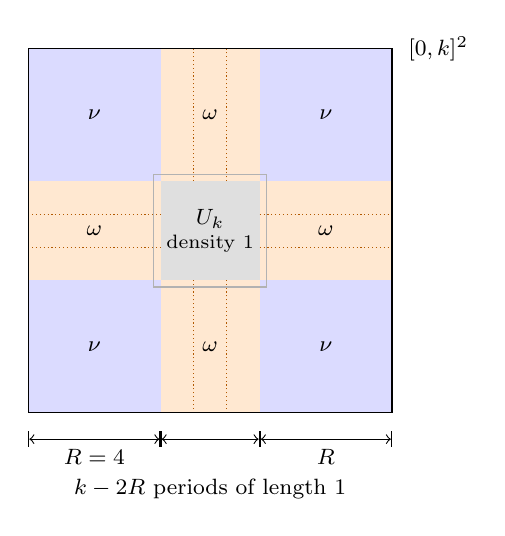
\begin{tikzpicture}[x=0.42cm,y=0.42cm,font=\footnotesize]
  % Lebesgue square U_k
  \fill[gray!25] (3.8,3.8) rectangle (7.2,7.2);
  % corner modules
  \foreach \x/\y in {0/0,7/0,0/7,7/7} \fill[blue!14] (\x,\y) rectangle ++(4,4);
  % wall pieces with their period-1 structure
  \fill[orange!18] (4,0) rectangle (7,4); \fill[orange!18] (4,7) rectangle (7,11);
  \fill[orange!18] (0,4) rectangle (4,7); \fill[orange!18] (7,4) rectangle (11,7);
  \foreach \t in {5,6} {\draw[orange!70!black,densely dotted] (\t,0)--(\t,4); \draw[orange!70!black,densely dotted] (\t,7)--(\t,11);
                        \draw[orange!70!black,densely dotted] (0,\t)--(4,\t); \draw[orange!70!black,densely dotted] (7,\t)--(11,\t);}
  \draw[gray!60] (3.8,3.8) rectangle (7.2,7.2);
  \draw (0,0) rectangle (11,11);
  \node at (2,2) {$\nu$}; \node at (9,2) {$\nu$}; \node at (2,9) {$\nu$}; \node at (9,9) {$\nu$};
  \node at (5.5,2) {$\omega$}; \node at (5.5,9) {$\omega$}; \node at (2,5.5) {$\omega$}; \node at (9,5.5) {$\omega$};
  \node[align=center] at (5.5,5.5) {$U_k$\\[-1pt]\scriptsize density $1$};
  % dimensions
  \draw[|<->|] (0,-0.8) -- node[below] {$R=4$} (4,-0.8);
  \draw[|<->|] (4,-0.8) -- (7,-0.8); \node[below] at (5.5,-1.7) {$k-2R$ periods of length $1$};
  \draw[|<->|] (7,-0.8) -- node[below] {$R$} (11,-0.8);
  \node[right] at (11.2,11) {$[0,k]^2$};
\end{tikzpicture}
